% !TEX root = ../thesis.tex

\chapter{Introduction}

\section{Liquid Crystals}
Liquid crystals are a special material which behaves between conventional liquids and solid crystals. They might flow like a liquid, but they preferred to be oriented in a crystal-like way. Historically, liquid crystals were discovered in 1888 when the Australian botanist Friedrich Reinitzer studied cholesterol benzoate, which is now known as cholesteric liquid crystals, and his friend German physicist Otto Lehmann named it "Liquid Crystal".

Overall liquid crystals can be classified into thermodynamic ones and lyotropic ones. The classification is according to the required condition of phase transition, thermodynamic liquid crystals undergo a phase transition as temperature is changed while the lyotropic liquid crystals undergo a phase transition as concentration is changed. In theoretical study we always use packing fraction instead of concentration. In natural environment they mainly consist of organic molecules and few minerals and in technological application they are more common, which can be used in electronic components or in liquid crystal displayers. They are also common in biology, for example tobacco mosaic virus, in which the ratio of length and thickness is around $15$.

Microscopically, liquid crystals are mostly rod-like or plate-like molecules, which enables them to behave anisotropically under certain circumstances. There are several typical phases which can arise under certain circumstances for a given molecule, and the schematic figure is given below.

\paragraph{Isotropic Phase}
Isotropic phases are the most common phases in any conventional liquid, this will happen if the temperature is too high (so that the kinetic energy dominates) or the density is too low (so that every molecule has much more space to move around). In any cases molecules can move freely regardless of its rod-like (or plate-like) shape, and they behaves just like conventional fluids.

\paragraph{Nematic Phase}
This is one of the most common anisotropic phase in liquid crystals. The term originates from Greek and means thread-like. Although the position of center of mass of them are still randomly distributed, they form a long-range directional order with their long axes nearly parallel. This always happens in relatively high density or low temperature condition (so that the interaction between molecules will dominate over kinetic energy). In this case molecules are pushing each other and tend to lean on each other in a nearly parallel way. The director (preferred direction) $n(r)$ is assumed to be invariant in the whole space in theoretical work.

\paragraph{Smectic Phase}
Smetic phase is observed in a much lower temperature than that of nematic phase, molecules are more ordered in this phase than that in nematic phase, they have a preferred direction as in nematic phase, and in addition the position of center of mass is ordered along one direction.

\paragraph{Cholesteric Phase}
It is more often called the chiral nematic phase, the name comes from the choleterol derivatives from which this phase was first observed. Only chiral molecules can give rise to such a phase. The chiral interaction between molecules will result in asymmetric packing, and further results in long-range chiral order. The twisting of molecules is perpendicular to local director. So there is a azimuthal twist between two layers, and on each layer the molecules behave like nematic phase, this is why is called the "chiral nematic phase". To be more precise theoretically, the director $n(r)$ in cholesteric phase is not invariant in the whole space, it is rotating along a direction perpendicular to itself. The distance between two layers over which the molecules undergo a $360^\circ$ twist, is the chiral pitch. The larger the chirality in molecule is, the smaller the pitch is.

\begin{figure}[H]
	\begin{minipage}{0.32\textwidth}
		\centering
		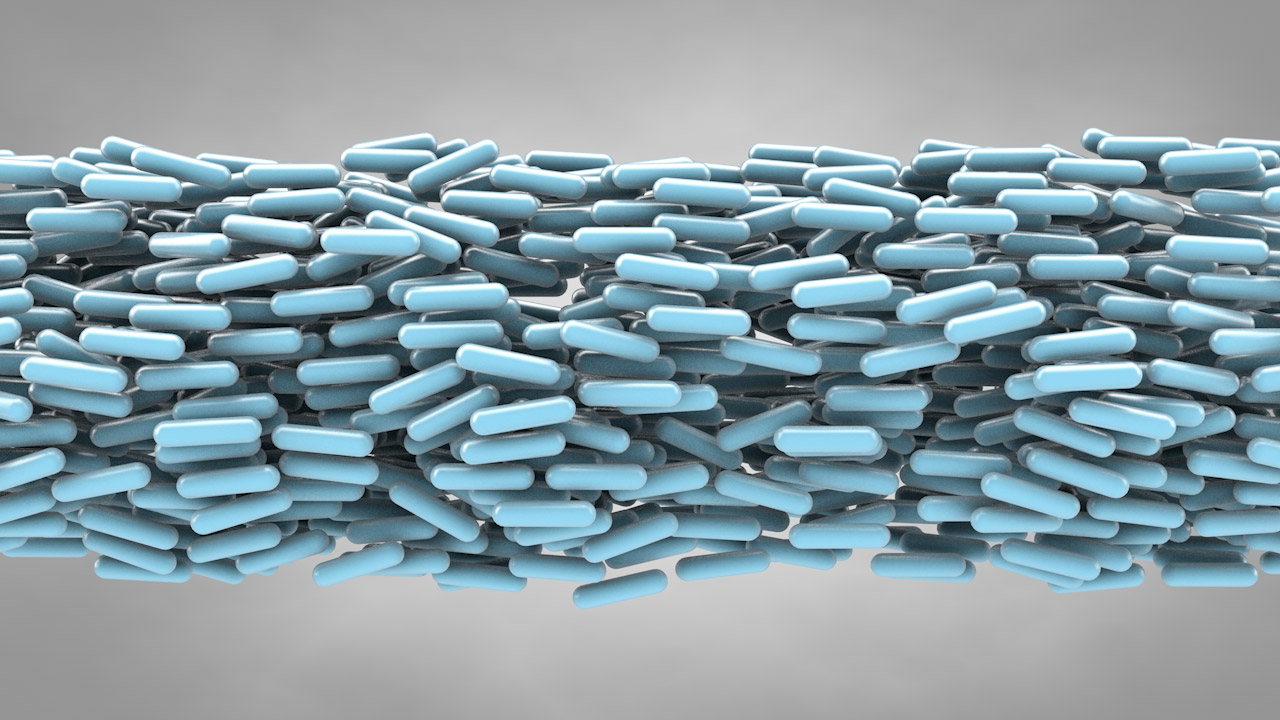
\includegraphics[width=\linewidth]{nematic.jpg}
		\caption{Nematic Phase}
		\label{fig:nematic}
	\end{minipage}
	\begin{minipage}{0.32\textwidth}
 		\centering
 		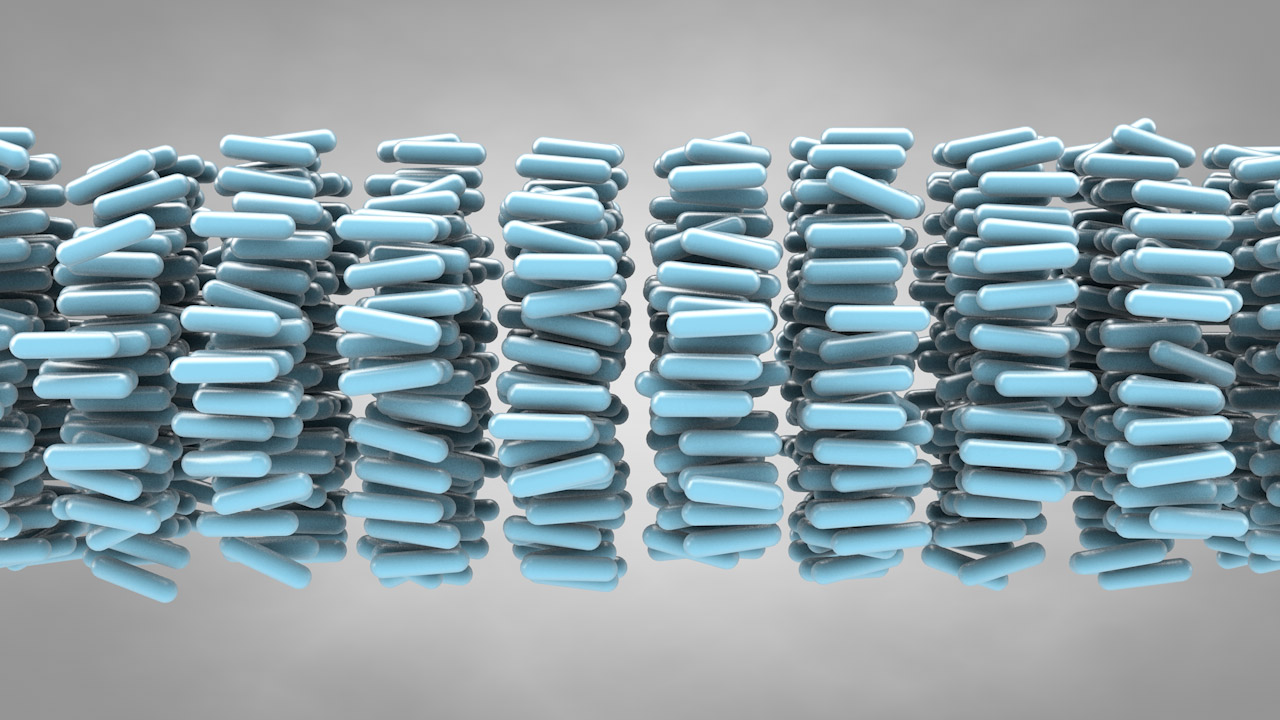
\includegraphics[width=\linewidth]{smectic.jpg}
 		\caption{Smectic Phase}
 		\label{fig:smetic}
 	\end{minipage}
 	\begin{minipage}{0.32\textwidth}
 		\centering
 		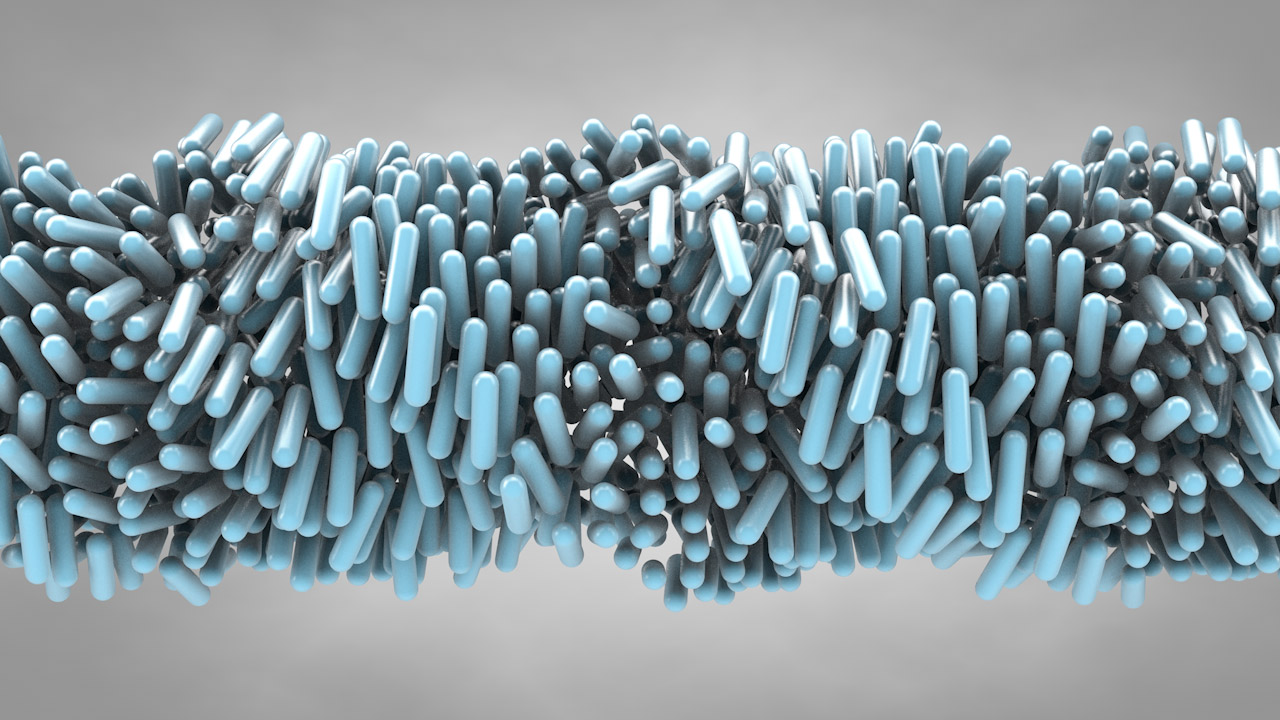
\includegraphics[width=\linewidth]{chiral.jpg}
 		\caption{Cholesteric Phase}
 		\label{fig:chiral}
 	\end{minipage}
\end{figure}

There are also other phases such as blue phase (which take place between cholesteric phase and isotropic phase), discotic phases and conic phases are also observed in various molecules, and we omit the detailed explanation here.

\section{Related Theoretical Work}

The theory of liquid crystal originates from Lars Onsager's seminar work\cite{Onsager1949NYAS} in 1949, to investigate how the phase transition happens and provide insight into the relationship between microscopic molecular characteristics and the macroscopic phase behavior, he considered the cylinders with large aspect ratio (the quotient of length and diameter $\kappa=L/D$), due to the spontaneous symmetry breaking in these kind of molecules, the distribution of orientation was not uniform, this is where the DFT theory come into play. He calculated the theoretical transition point of isotropic-nematic phase using Onsager's trial function. Oblate ($\kappa<1$) and prolate ($\kappa>1$) ellipsoids are also well-studied. In addition, the theories on soft\cite{Wu2014MM} and hard spherocylinders\cite{Jackson1996JCP} are also developed.

\begin{figure}[H]
 	\centering
 	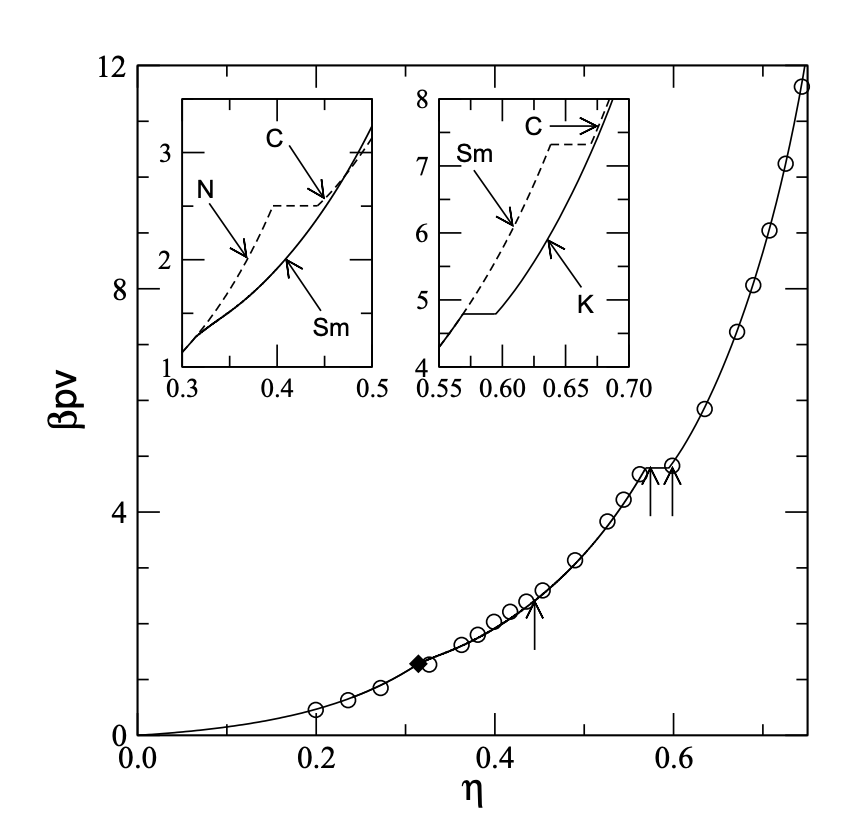
\includegraphics[width=\linewidth]{onsagerPhase.png}
	\caption[Phase Diagram of Hard Cylinders]{Phase diagram of Hard Cylinders\cite{Capit2008Phase}}
	\label{fig:fch}
\end{figure}

At the beginning of $20$th century, Born attributes the behavior of liquid crystals to the long-range electric interaction. Based on this viewpoint Maier and Saupe developed a phase transition theory, taking the dispersion forces between molecules and described the phase transition from isotropic to nematic. The Maier-Saupe theory provided a method which can effectively describe the temperature dependency and was used widely in thermodynamic liquid crystals. But the shape of the molecules which can significantly influence the anisotropicity of the molecule, was not taken care in the theory, so it was not suitable to describe lyotropic liquid crystals. Kimura combined Onsager's original model and dispersion forces, and described the isotropic-nematic phase transition by introducing the field of mean potential and a temperature-dependent order parameter. Further the dipole interactions are introduced, McGother used Monte Carlo method in canonical ensemble and simulated hard cylinders with dipole interactions, it turns out that in the case smetic phase was more likely to form than nematic phase. The series of studies showed that the phase behavior is in tight correlation with the long-range interactions (dispension forces, dipole interactions...)

This are also a number of ordinary cholesteric liquid crystals, the underlying reasons of their formation is still challenging. There are many research results showing that the long-range interaction is an important factor in the formation of cholesteric liquid crystals, for example, filamentous viruses\cite{35Dogic2006Ordered}, actins\cite{36Furukawa1993Formation}, cellulose derivatives\cite{37Werbowyj1980Ordered}, single-walled carbon nanotubes\cite{38Rai2007Dispersions}. There are also a lot of work on proposing a practical chiral-interaction between hard particles to reproduce the cholesteric phase, such as the Gossens model\cite{40Schoen2017Perturbation}, patchyrod model\cite{41Varga2006Study} (our FCh is one of these).

\section{Arrangement of The Thesis}

This undergraduate thesis mainly investigated electrically neutral lyotropic liquid crystals, this is a kind of typical soft matter. The understanding of liquid crystal at a molecular level is still challenging, in a preceding work by Liang\cite{Liang2017SM}, a coarse-grained molecular model is developed and represented by flexible chain with helical interactions (FCh). Since the molecular dynamics simulation is still limited by many factors, such as the different interactions involved, and the concrete simulation conditions. So developing general framework for predicting such liquid crystals is significant, as we will see in the following chapters, this general theoretical method can be applied to various kinds of liquid crystals and only take fewer time to predict the thermodynamic properties of certain molecules.

A theoretical method is developed in this thesis to give a prediction of thermodynamic properties of FCh model. The theory was based on Onsager's original theory of phase transition of liquid crystals, and made use of DFT method to give a depiction of the thermodynamic properties of the phase transition of FCh. In addition, a modular program is developed from scratch for the phase diagram computation of a wide range of liquid crystal molecules including FCh.

The thesis will first show introduce the DFT method in general case in Chap. \ref{chap:theory}, describing our theoretical method, we construct a theoretical framework to illustrate how the computation goes , in particular, we stated basic results in Onsager's original theory, which incorporates the ODF for the first time, and then introduce the Parsons-Lee's approximation, the method improves the original theory by a multiplicative coefficient, then Straley's approximation method is introduced when trying to find the cholesteric phase. Then we are going to study in Chap. \ref{chap:model} our molecular model and the existing simulation result, we further derive the thermodynamic properties of FCh by applying DFT method, and illustrating concrete Monte Carlo method involved in order to compute complicated integrals. We showed typical results and compared with simulation on the transition point isotropic-nematic phases.


